%
% $RCSfile: human_user.tex,v $
%
% Copyright (C) 2002-2008. Christian Heller.
%
% Permission is granted to copy, distribute and/or modify this document
% under the terms of the GNU Free Documentation License, Version 1.1 or
% any later version published by the Free Software Foundation; with no
% Invariant Sections, with no Front-Cover Texts and with no Back-Cover
% Texts. A copy of the license is included in the section entitled
% "GNU Free Documentation License".
%
% http://www.cybop.net
% - Cybernetics Oriented Programming -
%
% http://www.resmedicinae.org
% - Information in Medicine -
%
% Version: $Revision: 1.1 $ $Date: 2008-08-19 20:41:07 $ $Author: christian $
% Authors: Christian Heller <christian.heller@tuxtax.de>
%

\section{Human User}
\label{human_user_heading}
\index{Human User}
\index{Textual User Interface}
\index{TUI}
\index{Graphical User Interface}
\index{GUI}
\index{Human-Computer Interaction}
\index{HCI}

One system that needs special consideration is the \emph{Human User}. In the
first instance, it can be seen as normal system that is able to communicate
with other humans but also with artificial software systems running on machines
such as computers (figure \ref{user_figure}).

\begin{figure}[ht]
    \begin{center}
        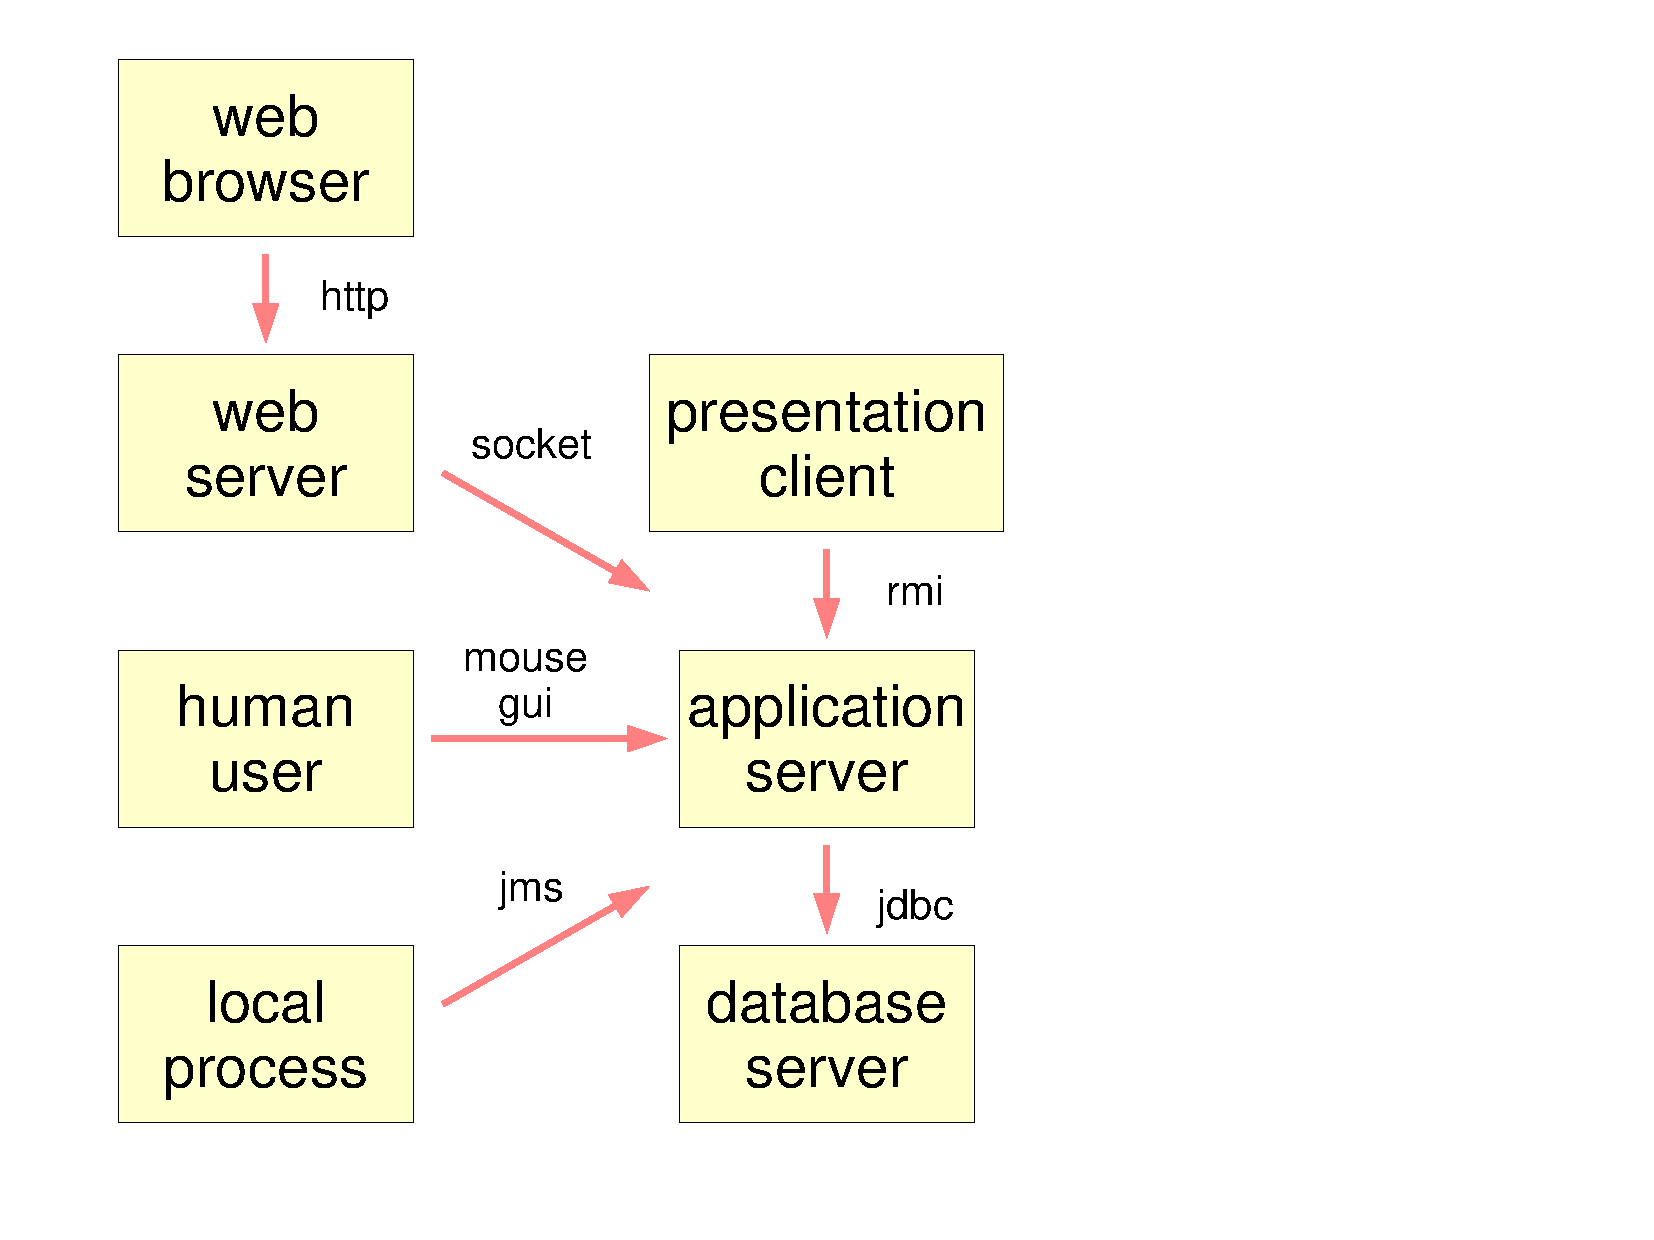
\includegraphics[scale=0.3,angle=-90]{graphic/user.pdf}
        \caption{Human User}
        \label{user_figure}
    \end{center}
\end{figure}

At the second view, one realises that due to the difference in construction,
human systems rely on other kinds of communication signals. While network cards
are usually enough for two computers to exchange data, additional input/ output
devices are needed to let human beings and computers talk to each other. To these
devices count: \emph{Keyboard}, \emph{Mouse}, \emph{Screen}, \emph{Printer} and
many more. They are made to suit the five human senses, that is to generate and
understand optical, acoustical, mechanical and similar signals.

The optical information displayed on a screen is often systematised into
character-based \emph{Textual User Interface} (TUI) and window-based
\emph{Graphical User Interface} (GUI).

The scientific subject dealing with those issues in more detail is called
\emph{Human-Computer Interaction} (HCI). One working definition given in
\cite{sigchi} states:

\begin{quote}
    Human-computer interaction is a discipline concerned with the design,
    evaluation and implementation of interactive computing systems for human
    use and with the study of major phenomena surrounding them.
\end{quote}
